\documentclass[
  coursetitle={Cómputo Nube y Tecnologías Emergentes},
  coursehours={96},
  coursedate={Verano 2026},
  doctype={Tutorial},
  otherlangs={english,french},
  authorname={Lázaro},
  authorsurname={Bustio-Martínez},
  authortitle={PhD},
  role={Profesor Investigador},
  email={lbustio@inaoe.mx},
  phone={5559504000},
  ext={7459},
  institution={Instituto Nacional de Astrofísica, Óptica y Electrónica (INAOE)},
  department={Maestría en Ciencias en Tecnologías de Seguridad},
  address={Luis Enrique Erro 1, Sta. Ma. Tonantzintla, San Andrés Cholula, CP 72840, Puebla, México},
  margin={0.5in}
]{../../lbustio_lecture_notes}

\usepackage[utf8]{inputenc}
\usepackage[T1]{fontenc}
\usepackage{array}
\usepackage{tabularx}
\usepackage{enumitem}
\usepackage{longtable}
\usepackage{booktabs}
\usepackage{url}
\usepackage{listings}
\usepackage{xcolor}
\usepackage{graphicx}
\usepackage{tcolorbox}
\usepackage{verbatim}
\usepackage{tikz}
\usetikzlibrary{arrows.meta,backgrounds,fit,positioning}

\definecolor{lightgray}{rgb}{0.97, 0.97, 0.97}
\definecolor{darkblue}{rgb}{0, 0, 0.6}
\definecolor{gcpblue}{HTML}{4285F4}
\definecolor{gcpgreen}{HTML}{34A853}
\definecolor{gcpyellow}{HTML}{FBBC04}
\definecolor{gcpred}{HTML}{EA4335}
\definecolor{softgray}{HTML}{F5F7FA}

\lstset{
  backgroundcolor=\color{lightgray},
  basicstyle=\ttfamily\small,
  breaklines=true,
  frame=single,
  columns=fullflexible,
  showstringspaces=false,
  commentstyle=\color{gray},
  keywordstyle=\color{darkblue},
  inputencoding=utf8,
  extendedchars=true,
  literate={á}{{\'a}}1 {é}{{\'e}}1 {í}{{\'i}}1 {ó}{{\'o}}1 {ú}{{\'u}}1 {ñ}{{\~n}}1
}

\setlist[itemize]{topsep=0.3em,itemsep=0.2em}
\setlist[enumerate]{topsep=0.3em,itemsep=0.2em}

\tikzset{
  cloudservice/.style={
    draw=gcpblue,
    fill=gcpblue!7,
    rounded corners=4pt,
    very thick,
    align=center,
    text width=0.62\textwidth,
    minimum height=1.15cm,
    inner sep=7pt
  },
  runtimeservice/.style={
    cloudservice,
    draw=gcpgreen,
    fill=gcpgreen!9
  },
  modelservice/.style={
    cloudservice,
    draw=gcpyellow!80!black,
    fill=gcpyellow!14
  },
  apiservice/.style={
    cloudservice,
    draw=gcpred,
    fill=gcpred!7
  },
  compactservice/.style={
    draw=gcpblue,
    fill=softgray,
    rounded corners=4pt,
    thick,
    align=center,
    text width=3.2cm,
    minimum height=1.0cm,
    inner sep=5pt
  },
  pipestage/.style={
    draw=gcpblue,
    fill=gcpblue!7,
    rounded corners=4pt,
    thick,
    align=center,
    text width=3.45cm,
    minimum height=0.95cm,
    inner sep=5pt
  },
  flowarrow/.style={
    -{Latex[length=3mm,width=2mm]},
    thick,
    draw=darkblue
  }
}

\begin{document}

\IberoCover

%\begin{center}
%    \vspace{0.5cm}
%    \LARGE \textbf{Guía de Laboratorio Operativo y Reproducible} \\
%    \vspace{0.3cm}
%    \huge \textbf{Aprendizaje Automatizado en Google Cloud Platform}
%    \vspace{0.5cm}
%\end{center}

\section{Objetivo de la práctica}

El objetivo de esta práctica es construir un flujo completo de Machine Learning en Google Cloud Platform (GCP), desde el almacenamiento de datos hasta el despliegue de un modelo como servicio web.

Al finalizar la práctica, el estudiante será capaz de:

\begin{itemize}
    \item utilizar Cloud Storage para almacenar datasets;
    \item utilizar Colab Enterprise como entorno de desarrollo;
    \item cargar datos desde Cloud Storage;
    \item preparar datos para Machine Learning;
    \item entrenar un modelo supervisado;
    \item evaluar el desempeño del modelo;
    \item guardar un modelo entrenado;
    \item almacenar el modelo en Cloud Storage;
    \item desplegar el modelo mediante Cloud Run;
    \item consumir el modelo a través de una API REST.
\end{itemize}

\section{Arquitectura de la solución}

La práctica sigue una arquitectura mínima, reproducible y orientada al aprendizaje. El dataset se almacena en Cloud Storage, el entrenamiento ocurre en Colab Enterprise y el modelo resultante se despliega como servicio HTTP mediante Cloud Run.

\begin{center}
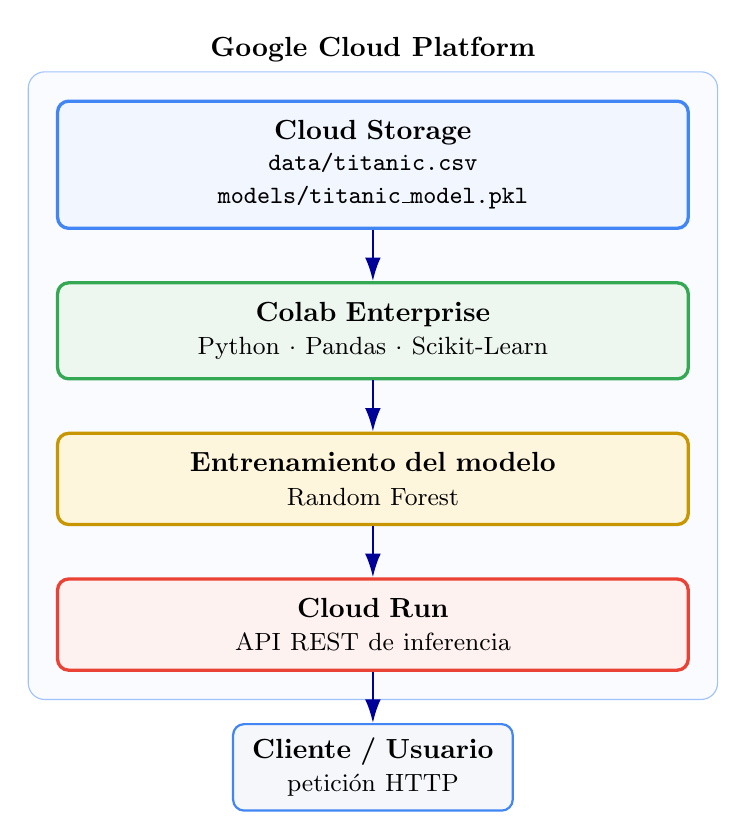
\begin{tikzpicture}[node distance=0.65cm]
    \node[cloudservice] (storage) {
        \textbf{Cloud Storage}\\
        \small \texttt{data/titanic.csv}\\
        \small \texttt{models/titanic\_model.pkl}
    };
    \node[runtimeservice, below=of storage] (colab) {
        \textbf{Colab Enterprise}\\
        \small Python \(\cdot\) Pandas \(\cdot\) Scikit-Learn
    };
    \node[modelservice, below=of colab] (training) {
        \textbf{Entrenamiento del modelo}\\
        \small Random Forest
    };
    \node[apiservice, below=of training] (cloudrun) {
        \textbf{Cloud Run}\\
        \small API REST de inferencia
    };
    \node[compactservice, below=of cloudrun] (client) {
        \textbf{Cliente / Usuario}\\
        \small petición HTTP
    };

    \draw[flowarrow] (storage) -- (colab);
    \draw[flowarrow] (colab) -- (training);
    \draw[flowarrow] (training) -- (cloudrun);
    \draw[flowarrow] (cloudrun) -- (client);

    \begin{scope}[on background layer]
        \node[
            draw=gcpblue!50,
            fill=gcpblue!3,
            rounded corners=6pt,
            inner sep=10pt,
            fit=(storage)(colab)(training)(cloudrun),
            label={[font=\bfseries]above:Google Cloud Platform}
        ] {};
    \end{scope}
\end{tikzpicture}

\small\textbf{Figura:} Arquitectura general del flujo de Machine Learning en GCP.
\end{center}

\section{Tecnologías utilizadas}

\subsection{Google Cloud Platform}

Google Cloud Platform (GCP) es la plataforma de computación en la nube desarrollada por Google. Proporciona infraestructura, almacenamiento, inteligencia artificial, redes y servicios administrados.

\subsection{Cloud Storage}

Cloud Storage es el servicio de almacenamiento de objetos de Google Cloud. En esta práctica se utilizará para almacenar:

\begin{itemize}
    \item el dataset Titanic;
    \item el modelo entrenado.
\end{itemize}

\subsection{Colab Enterprise}

Colab Enterprise es un entorno administrado basado en notebooks Jupyter. En esta práctica se utilizará para:

\begin{itemize}
    \item ejecutar código Python;
    \item analizar datos;
    \item entrenar modelos;
    \item evaluar resultados.
\end{itemize}

\subsection{Python}

Python será el lenguaje de programación utilizado para implementar todo el flujo de trabajo.

\subsection{Pandas}

Pandas es una biblioteca especializada en manipulación y análisis de datos. Se utilizará para cargar, explorar y preparar el dataset.

\subsection{Scikit-Learn}

Scikit-Learn es una biblioteca de Machine Learning que se utilizará para:

\begin{itemize}
    \item dividir datos;
    \item entrenar el modelo;
    \item evaluar resultados;
    \item generar predicciones.
\end{itemize}

\subsection{Cloud Run}

Cloud Run es un servicio serverless utilizado para desplegar aplicaciones contenidas en Docker. En esta práctica se usará para publicar una API de inferencia.

\section{Preparación del proyecto}

Antes de iniciar el laboratorio, realice las siguientes verificaciones:

\begin{enumerate}
    \item Acceda a Google Cloud Console.
    \item Seleccione el proyecto de trabajo.
    \item Verifique que la facturación se encuentre habilitada.
    \item Verifique que estén disponibles los siguientes servicios:
\end{enumerate}

\begin{itemize}
    \item Cloud Storage;
    \item Colab Enterprise;
    \item Cloud Run;
    \item Artifact Registry;
    \item Cloud Build.
\end{itemize}

\section{Creación del bucket}

Desde Google Cloud Console, navegue a:

\begin{center}
    \textit{Cloud Storage} \(\rightarrow\) \textit{Buckets} \(\rightarrow\) \textit{Crear bucket}
\end{center}

Asigne un nombre único al bucket. Para efectos de esta guía se utilizará el siguiente nombre de ejemplo:

\begin{lstlisting}
titanic-tutorial
\end{lstlisting}

Una vez creado el bucket, genere la siguiente estructura lógica:

\begin{lstlisting}
data/
models/
\end{lstlisting}

Suba el dataset en la siguiente ruta:

\begin{lstlisting}
data/titanic.csv
\end{lstlisting}

\textbf{Resultado esperado:} El bucket debe contener el archivo \texttt{data/titanic.csv}.

\section{Creación del notebook}

Desde Google Cloud Console, navegue a:

\begin{center}
    \textit{Plataforma de agentes} \(\rightarrow\) \textit{Notebooks} \(\rightarrow\) \textit{Colab Enterprise}
\end{center}

Cree un notebook nuevo con el siguiente nombre sugerido:

\begin{lstlisting}
Titanic_ML_GCP
\end{lstlisting}

\section{Verificación del entorno}

Verifique la versión de Python disponible en el runtime:

\begin{lstlisting}
import sys

print(sys.version)
\end{lstlisting}

Verifique también que estén disponibles las bibliotecas principales:

\begin{lstlisting}
import pandas as pd
import sklearn

print("Pandas:", pd.__version__)
print("Scikit-Learn:", sklearn.__version__)
\end{lstlisting}

\section{Dónde se ejecuta el notebook}

Aunque el notebook se abre desde el navegador, el código no se ejecuta en la computadora local. El navegador únicamente muestra la interfaz. La ejecución real ocurre dentro de un runtime administrado por Google Cloud.

\begin{center}
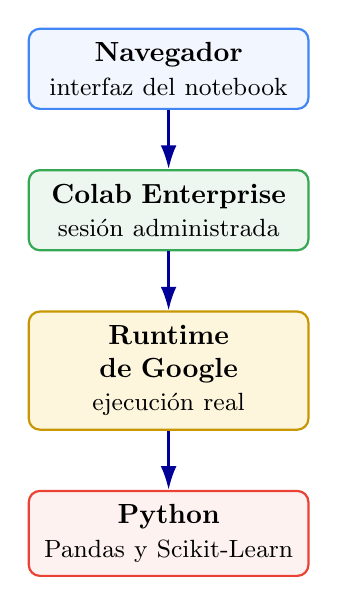
\begin{tikzpicture}[node distance=0.75cm]
    \node[compactservice, draw=gcpblue, fill=gcpblue!7] (browser) {
        \textbf{Navegador}\\
        \small interfaz del notebook
    };
    \node[compactservice, draw=gcpgreen, fill=gcpgreen!9, below=of browser] (colabui) {
        \textbf{Colab Enterprise}\\
        \small sesión administrada
    };
    \node[compactservice, draw=gcpyellow!80!black, fill=gcpyellow!14, below=of colabui] (runtime) {
        \textbf{Runtime de Google}\\
        \small ejecución real
    };
    \node[compactservice, draw=gcpred, fill=gcpred!7, below=of runtime] (python) {
        \textbf{Python}\\
        \small Pandas y Scikit-Learn
    };

    \draw[flowarrow] (browser) -- (colabui);
    \draw[flowarrow] (colabui) -- (runtime);
    \draw[flowarrow] (runtime) -- (python);
\end{tikzpicture}

\small\textbf{Figura:} Separación entre la interfaz web y el entorno real de ejecución.
\end{center}

Verifique el entorno desde una celda del notebook:

\begin{lstlisting}
!hostname
!nproc
!free -h
\end{lstlisting}

\begin{tcolorbox}[title=Conclusión operativa]
El dataset vive en Cloud Storage, el código vive en el notebook, la ejecución ocurre en Colab Enterprise y los archivos locales del runtime son temporales.
\end{tcolorbox}

\section{Carga del dataset}

Importe Pandas:

\begin{lstlisting}
import pandas as pd
\end{lstlisting}

Cargue el archivo desde Cloud Storage:

\begin{lstlisting}
df = pd.read_csv(
    "gs://titanic-tutorial/data/titanic.csv"
)
\end{lstlisting}

Muestre los primeros registros:

\begin{lstlisting}
df.head()
\end{lstlisting}

Verifique las dimensiones del dataset:

\begin{lstlisting}
df.shape
\end{lstlisting}

Muestre las columnas disponibles:

\begin{lstlisting}
df.columns
\end{lstlisting}

Obtenga información general sobre los tipos de datos y valores faltantes:

\begin{lstlisting}
df.info()
\end{lstlisting}

\section{Comprensión del problema}

El objetivo del modelo es predecir la supervivencia de pasajeros del Titanic.

\begin{description}
    \item[Variable objetivo:] \texttt{Survived}
    \item[Valor 0:] el pasajero no sobrevivió.
    \item[Valor 1:] el pasajero sobrevivió.
\end{description}

\section{Preparación de los datos}

Defina la variable objetivo:

\begin{lstlisting}
y = df["Survived"]
\end{lstlisting}

Seleccione las variables predictoras:

\begin{lstlisting}
X = df[
    [
        "Pclass",
        "Sex",
        "Age",
        "SibSp",
        "Parch",
        "Fare"
    ]
]
\end{lstlisting}

Revise los valores faltantes:

\begin{lstlisting}
X.isnull().sum()
\end{lstlisting}

Rellene las edades faltantes usando la mediana:

\begin{lstlisting}
X["Age"] = X["Age"].fillna(
    X["Age"].median()
)
\end{lstlisting}

Transforme la variable categórica \texttt{Sex} a valores numéricos:

\begin{lstlisting}
X["Sex"] = X["Sex"].map(
    {
        "male": 0,
        "female": 1
    }
)
\end{lstlisting}

Verifique el resultado:

\begin{lstlisting}
X.head()
\end{lstlisting}

\section{División entrenamiento/prueba}

Importe la función de división de datos:

\begin{lstlisting}
from sklearn.model_selection import train_test_split
\end{lstlisting}

Divida los datos en entrenamiento y prueba:

\begin{lstlisting}
X_train, X_test, y_train, y_test = train_test_split(
    X,
    y,
    test_size=0.2,
    random_state=42
)
\end{lstlisting}

Verifique los tamaños de ambos subconjuntos:

\begin{lstlisting}
print(X_train.shape)
print(X_test.shape)
\end{lstlisting}

\section{Entrenamiento del modelo}

Importe el algoritmo:

\begin{lstlisting}
from sklearn.ensemble import RandomForestClassifier
\end{lstlisting}

Cree el modelo:

\begin{lstlisting}
model = RandomForestClassifier(
    n_estimators=100,
    random_state=42
)
\end{lstlisting}

Entrene el modelo:

\begin{lstlisting}
model.fit(
    X_train,
    y_train
)
\end{lstlisting}

Genere predicciones sobre el conjunto de prueba:

\begin{lstlisting}
y_pred = model.predict(X_test)
\end{lstlisting}

Revise las primeras predicciones:

\begin{lstlisting}
y_pred[:10]
\end{lstlisting}

\section{Evaluación del modelo}

Calcule el accuracy:

\begin{lstlisting}
from sklearn.metrics import accuracy_score

accuracy = accuracy_score(
    y_test,
    y_pred
)

print(f"Accuracy: {accuracy:.4f}")
\end{lstlisting}

Calcule la matriz de confusión:

\begin{lstlisting}
from sklearn.metrics import confusion_matrix

cm = confusion_matrix(
    y_test,
    y_pred
)

print(cm)
\end{lstlisting}

Visualice la matriz de confusión:

\begin{lstlisting}
from sklearn.metrics import ConfusionMatrixDisplay
import matplotlib.pyplot as plt

ConfusionMatrixDisplay(cm).plot()

plt.show()
\end{lstlisting}

\section{Importancia de variables}

Construya una tabla con la importancia de cada variable:

\begin{lstlisting}
importance = pd.DataFrame(
    {
        "Variable": X.columns,
        "Importance": model.feature_importances_
    }
)

importance.sort_values(
    "Importance",
    ascending=False
)
\end{lstlisting}

Preguntas de análisis:

\begin{itemize}
    \item ¿Qué variable fue la más importante?
    \item ¿Qué variable fue la menos importante?
\end{itemize}

\section{Predicción sobre un nuevo pasajero}

Cree un registro nuevo con los atributos de un pasajero hipotético:

\begin{lstlisting}
new_passenger = pd.DataFrame(
    {
        "Pclass": [1],
        "Sex": [1],
        "Age": [25],
        "SibSp": [0],
        "Parch": [0],
        "Fare": [100]
    }
)
\end{lstlisting}

Genere la predicción:

\begin{lstlisting}
prediction = model.predict(
    new_passenger
)

print(prediction)
\end{lstlisting}

Obtenga las probabilidades asociadas a cada clase:

\begin{lstlisting}
probability = model.predict_proba(
    new_passenger
)

print(probability)
\end{lstlisting}

\section{Guardado del modelo}

Importe \texttt{joblib} y serialice el modelo entrenado:

\begin{lstlisting}
import joblib

joblib.dump(
    model,
    "titanic_model.pkl"
)
\end{lstlisting}

Verifique que el archivo fue creado:

\begin{lstlisting}
import os

os.path.exists(
    "titanic_model.pkl"
)
\end{lstlisting}

\section{Subida del modelo a Cloud Storage}

Importe el cliente de Cloud Storage:

\begin{lstlisting}
from google.cloud import storage
\end{lstlisting}

Configure el bucket de trabajo:

\begin{lstlisting}
bucket_name = "titanic-tutorial"

storage_client = storage.Client()

bucket = storage_client.bucket(
    bucket_name
)
\end{lstlisting}

Prepare el objeto remoto y suba el modelo:

\begin{lstlisting}
blob = bucket.blob(
    "models/titanic_model.pkl"
)

blob.upload_from_filename(
    "titanic_model.pkl"
)

print(
    "Modelo subido correctamente"
)
\end{lstlisting}

\textbf{Resultado esperado:} El bucket debe contener los siguientes objetos:

\begin{lstlisting}
data/titanic.csv
models/titanic_model.pkl
\end{lstlisting}

\section{Despliegue del modelo}

El objetivo de esta fase es convertir el modelo entrenado en una API REST. La arquitectura lógica del servicio será:

\begin{center}
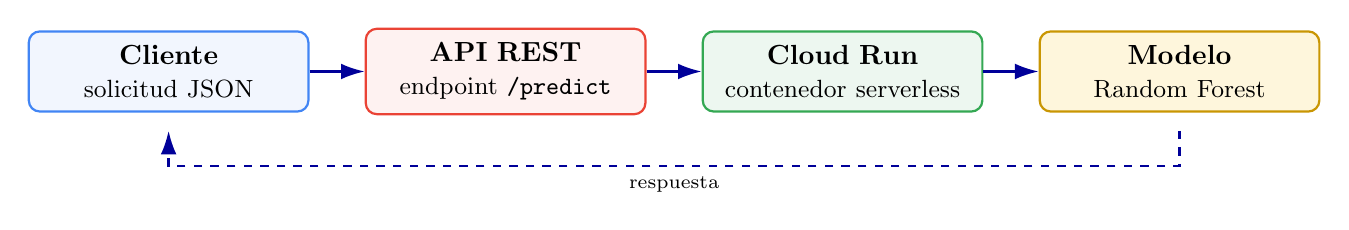
\begin{tikzpicture}[node distance=0.7cm]
    \node[compactservice, draw=gcpblue, fill=gcpblue!7] (client) {
        \textbf{Cliente}\\
        \small solicitud JSON
    };
    \node[compactservice, draw=gcpred, fill=gcpred!7, right=of client] (api) {
        \textbf{API REST}\\
        \small endpoint \texttt{/predict}
    };
    \node[compactservice, draw=gcpgreen, fill=gcpgreen!9, right=of api] (run) {
        \textbf{Cloud Run}\\
        \small contenedor serverless
    };
    \node[compactservice, draw=gcpyellow!80!black, fill=gcpyellow!14, right=of run] (model) {
        \textbf{Modelo}\\
        \small Random Forest
    };

    \draw[flowarrow] (client) -- (api);
    \draw[flowarrow] (api) -- (run);
    \draw[flowarrow] (run) -- (model);
    \draw[flowarrow, dashed] ([yshift=-0.23cm]model.south) -- ++(0,-0.45) -| node[pos=0.25, below, font=\scriptsize] {respuesta} ([yshift=-0.23cm]client.south);
\end{tikzpicture}

\small\textbf{Figura:} Ruta lógica de una solicitud de inferencia desplegada en Cloud Run.
\end{center}

\section{Creación de app.py}

Cree el archivo \texttt{app.py} con el siguiente contenido:

\begin{lstlisting}
from flask import Flask, request, jsonify
import pandas as pd
import joblib
from google.cloud import storage
import os

app = Flask(__name__)

BUCKET_NAME = "titanic-tutorial"
MODEL_BLOB_PATH = "models/titanic_model.pkl"
LOCAL_MODEL_PATH = "/tmp/titanic_model.pkl"

def download_model():
    storage_client = storage.Client()
    bucket = storage_client.bucket(BUCKET_NAME)
    blob = bucket.blob(MODEL_BLOB_PATH)
    blob.download_to_filename(LOCAL_MODEL_PATH)

download_model()

model = joblib.load(LOCAL_MODEL_PATH)

@app.route("/", methods=["GET"])
def health_check():
    return jsonify({"status": "ok"})

@app.route("/predict", methods=["POST"])
def predict():

    data = request.get_json()

    input_data = pd.DataFrame([{
        "Pclass": data["Pclass"],
        "Sex": data["Sex"],
        "Age": data["Age"],
        "SibSp": data["SibSp"],
        "Parch": data["Parch"],
        "Fare": data["Fare"]
    }])

    prediction = model.predict(input_data)[0]

    probability = model.predict_proba(
        input_data
    )[0].tolist()

    return jsonify({
        "prediction": int(prediction),
        "probability_no_survived": probability[0],
        "probability_survived": probability[1]
    })

if __name__ == "__main__":
    port = int(
        os.environ.get("PORT", 8080)
    )

    app.run(
        host="0.0.0.0",
        port=port
    )
\end{lstlisting}

\section{Creación de requirements.txt}

Cree el archivo \texttt{requirements.txt} con las dependencias de la API:

\begin{lstlisting}
flask
pandas
scikit-learn
joblib
google-cloud-storage
gunicorn
\end{lstlisting}

\section{Creación del Dockerfile}

Cree el archivo \texttt{Dockerfile} con el siguiente contenido:

\begin{lstlisting}
FROM python:3.11-slim

WORKDIR /app

COPY requirements.txt .

RUN pip install \
    --no-cache-dir \
    -r requirements.txt

COPY app.py .

CMD exec gunicorn \
    --bind :$PORT \
    --workers 1 \
    --threads 8 \
    app:app
\end{lstlisting}

\section{Despliegue en Cloud Run}

Desde el directorio que contiene \texttt{app.py}, \texttt{requirements.txt} y \texttt{Dockerfile}, ejecute:

\begin{lstlisting}
gcloud run deploy titanic-ml-api \
    --source . \
    --region us-central1 \
    --allow-unauthenticated
\end{lstlisting}

Espere a que finalice el despliegue. Cloud Run devolverá una URL pública para consumir el servicio.

\section{Prueba del servicio}

Verifique el estado de la API:

\begin{lstlisting}
curl https://URL_DEL_SERVICIO
\end{lstlisting}

\textbf{Resultado esperado:}

\begin{lstlisting}
{"status":"ok"}
\end{lstlisting}

Realice una predicción:

\begin{lstlisting}
curl -X POST \
"https://URL_DEL_SERVICIO/predict" \
-H "Content-Type: application/json" \
-d '{
    "Pclass":1,
    "Sex":1,
    "Age":25,
    "SibSp":0,
    "Parch":0,
    "Fare":100
}'
\end{lstlisting}

\textbf{Resultado esperado:}

\begin{lstlisting}
{
  "prediction": 1,
  "probability_no_survived": 0.02,
  "probability_survived": 0.98
}
\end{lstlisting}

\section{Conclusiones}

En esta práctica se implementó un flujo completo de Machine Learning en Google Cloud Platform:

\begin{center}
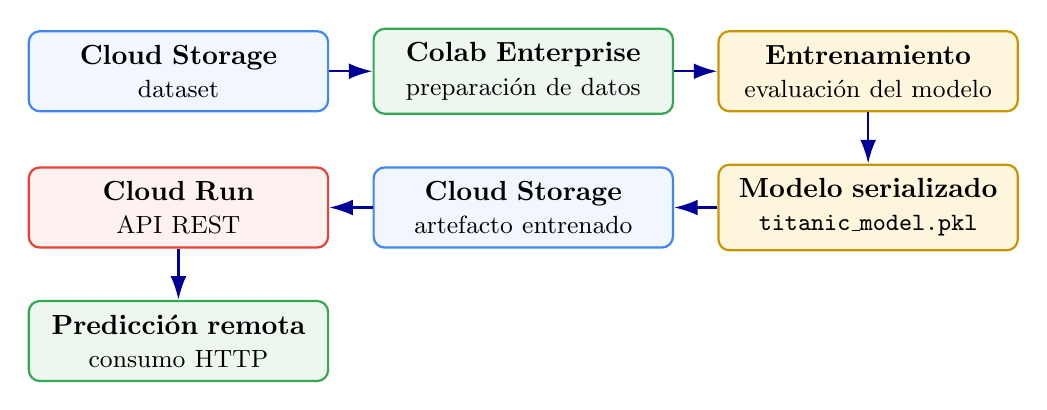
\begin{tikzpicture}[node distance=0.65cm and 0.55cm]
    \node[pipestage, draw=gcpblue, fill=gcpblue!7] (storagein) {
        \textbf{Cloud Storage}\\
        \small dataset
    };
    \node[pipestage, draw=gcpgreen, fill=gcpgreen!9, right=of storagein] (colabflow) {
        \textbf{Colab Enterprise}\\
        \small preparación de datos
    };
    \node[pipestage, draw=gcpyellow!80!black, fill=gcpyellow!14, right=of colabflow] (trainflow) {
        \textbf{Entrenamiento}\\
        \small evaluación del modelo
    };
    \node[pipestage, draw=gcpyellow!80!black, fill=gcpyellow!14, below=of trainflow] (serialized) {
        \textbf{Modelo serializado}\\
        \small \texttt{titanic\_model.pkl}
    };
    \node[pipestage, draw=gcpblue, fill=gcpblue!7, left=of serialized] (storageout) {
        \textbf{Cloud Storage}\\
        \small artefacto entrenado
    };
    \node[pipestage, draw=gcpred, fill=gcpred!7, left=of storageout] (cloudrunflow) {
        \textbf{Cloud Run}\\
        \small API REST
    };
    \node[pipestage, draw=gcpgreen, fill=gcpgreen!9, below=of cloudrunflow] (prediction) {
        \textbf{Predicción remota}\\
        \small consumo HTTP
    };

    \draw[flowarrow] (storagein) -- (colabflow);
    \draw[flowarrow] (colabflow) -- (trainflow);
    \draw[flowarrow] (trainflow) -- (serialized);
    \draw[flowarrow] (serialized) -- (storageout);
    \draw[flowarrow] (storageout) -- (cloudrunflow);
    \draw[flowarrow] (cloudrunflow) -- (prediction);
\end{tikzpicture}

\small\textbf{Figura:} Pipeline completo de datos, entrenamiento, despliegue y consumo remoto.
\end{center}

Este flujo representa una arquitectura simplificada de producción utilizada en numerosas aplicaciones modernas de Inteligencia Artificial.

\end{document}
